\documentclass[12pt,a4paper]{article}
\usepackage[utf8]{inputenc}
\usepackage{amsmath}
\usepackage{amsfonts}
\usepackage{amssymb}
\usepackage{graphicx}
\usepackage{lmodern}
\usepackage{kpfonts}
\author{Andrea Colarieti Tosti}
\title{Rechenarchitektur Übungblatt 3 Lösung}

\begin{document}
\maketitle
\newpage

\section{Aufgabe 13}
\subsection{a}

\begin{tabular}{|c|c|c||c|c|c|}
\hline
a & b & c & G & O & R \\
\hline
1	&	1	&	1	&	0	&	0	&	1	\\
\hline
1	&	1	&	0	&	0	&	1	&	0	\\
\hline
1	&	0	&	1	&	0	&	1	&	0	\\
\hline
1	&	0	&	0	&	1	&	0	&	0	\\
\hline
0	&	1	&	1	&	0	&	1	&	0	\\
\hline
0	&	1	&	0	&	1	&	0	&	0	\\
\hline
0	&	0	&	1	&	1	&	0	&	0	\\
\hline
0	&	0	&	0	&	0	&	1	&	0	\\
\hline
\end{tabular}

\subsection{b}
$ G(a,b,c)= (a\overline{b}\overline{c})+(\overline{a}b\overline{c})+(\overline{a}\overline{b}c)$
\subsection{c}
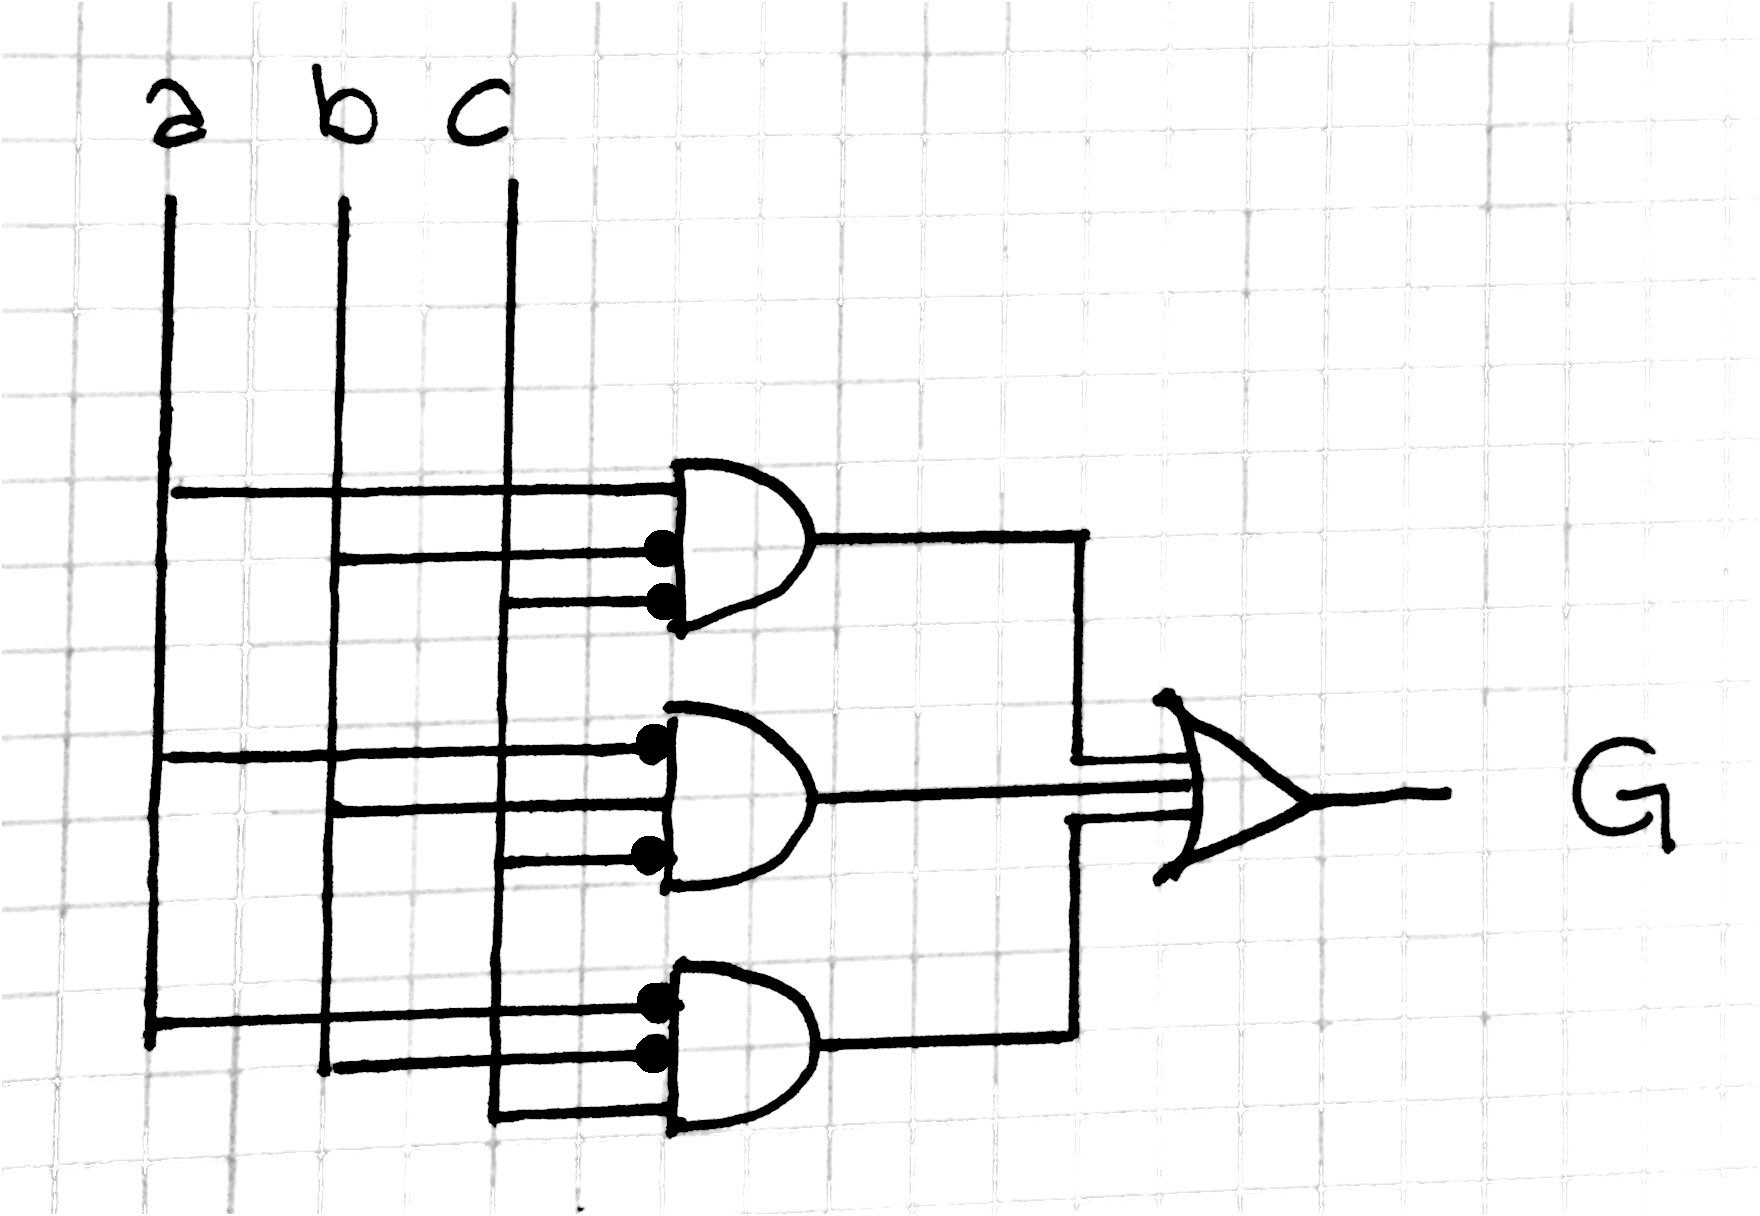
\includegraphics[scale=0.21]{a.jpg} 

\newpage
\section{Aufgabe 15}
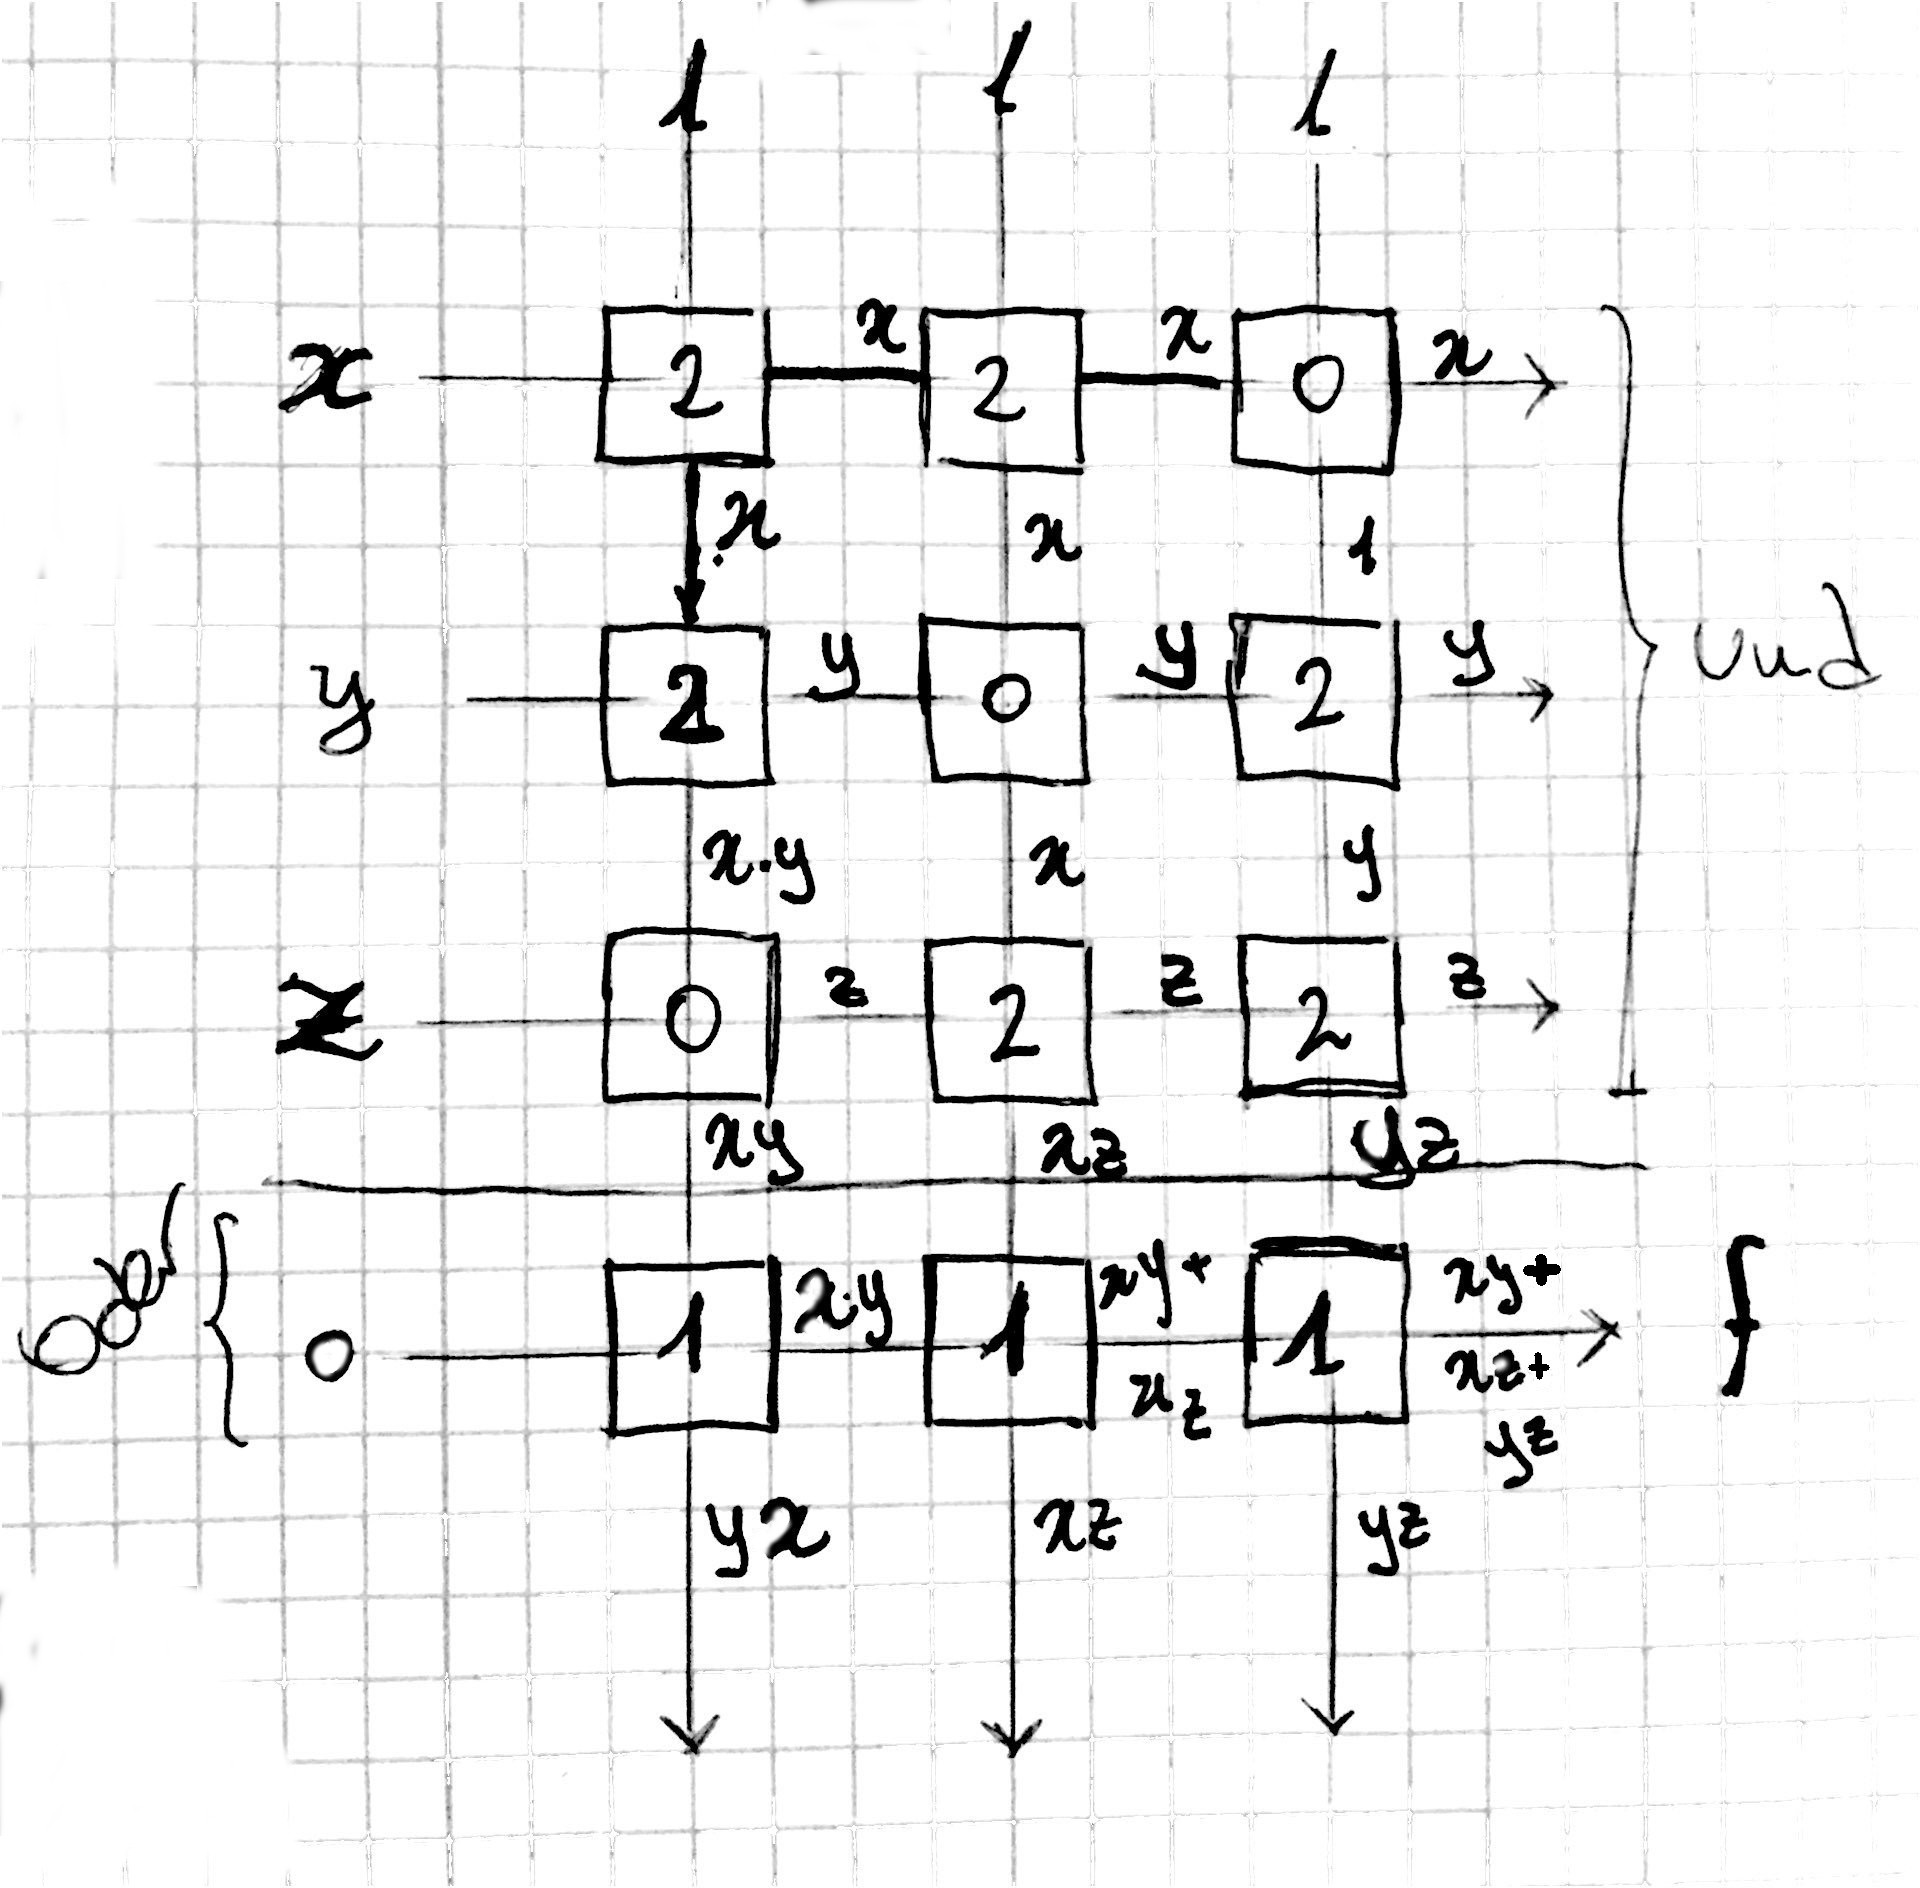
\includegraphics[scale=0.21]{b.jpg} 

\newpage
\section{Aufgabe 16}
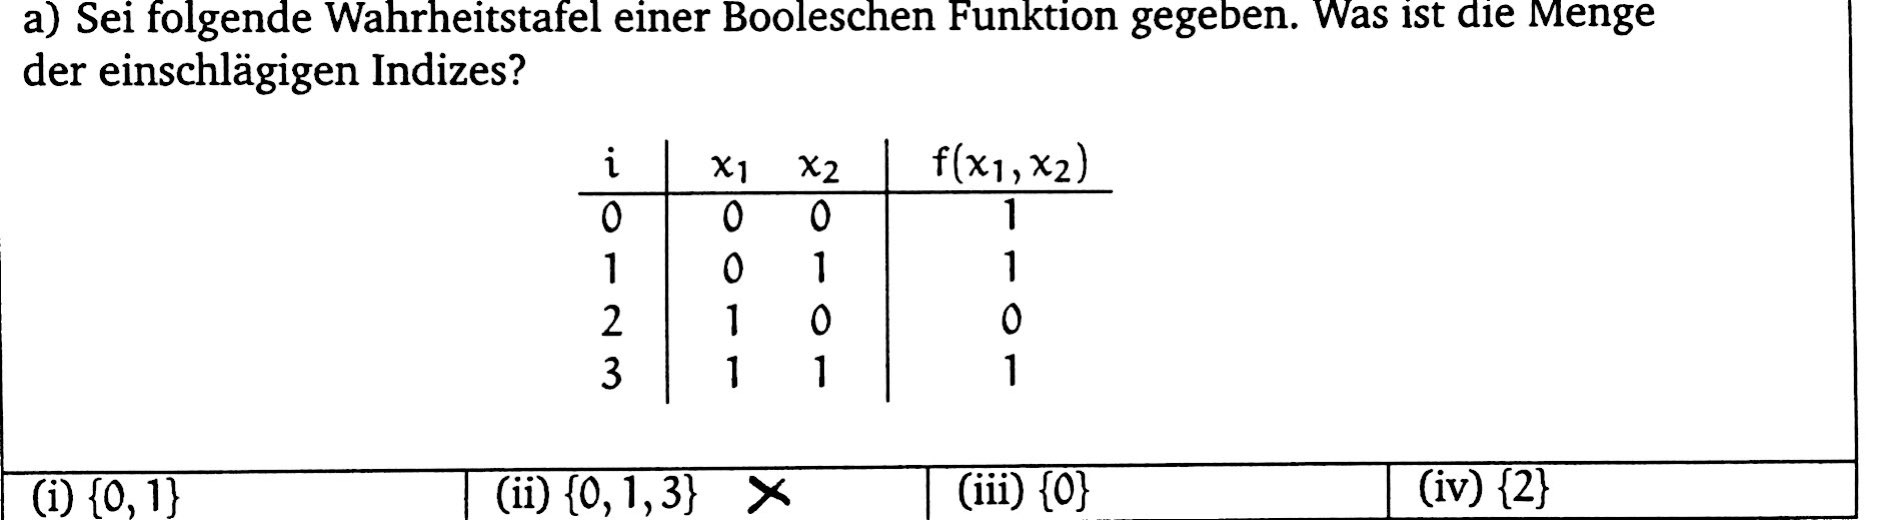
\includegraphics[scale=0.21]{c.jpg} 
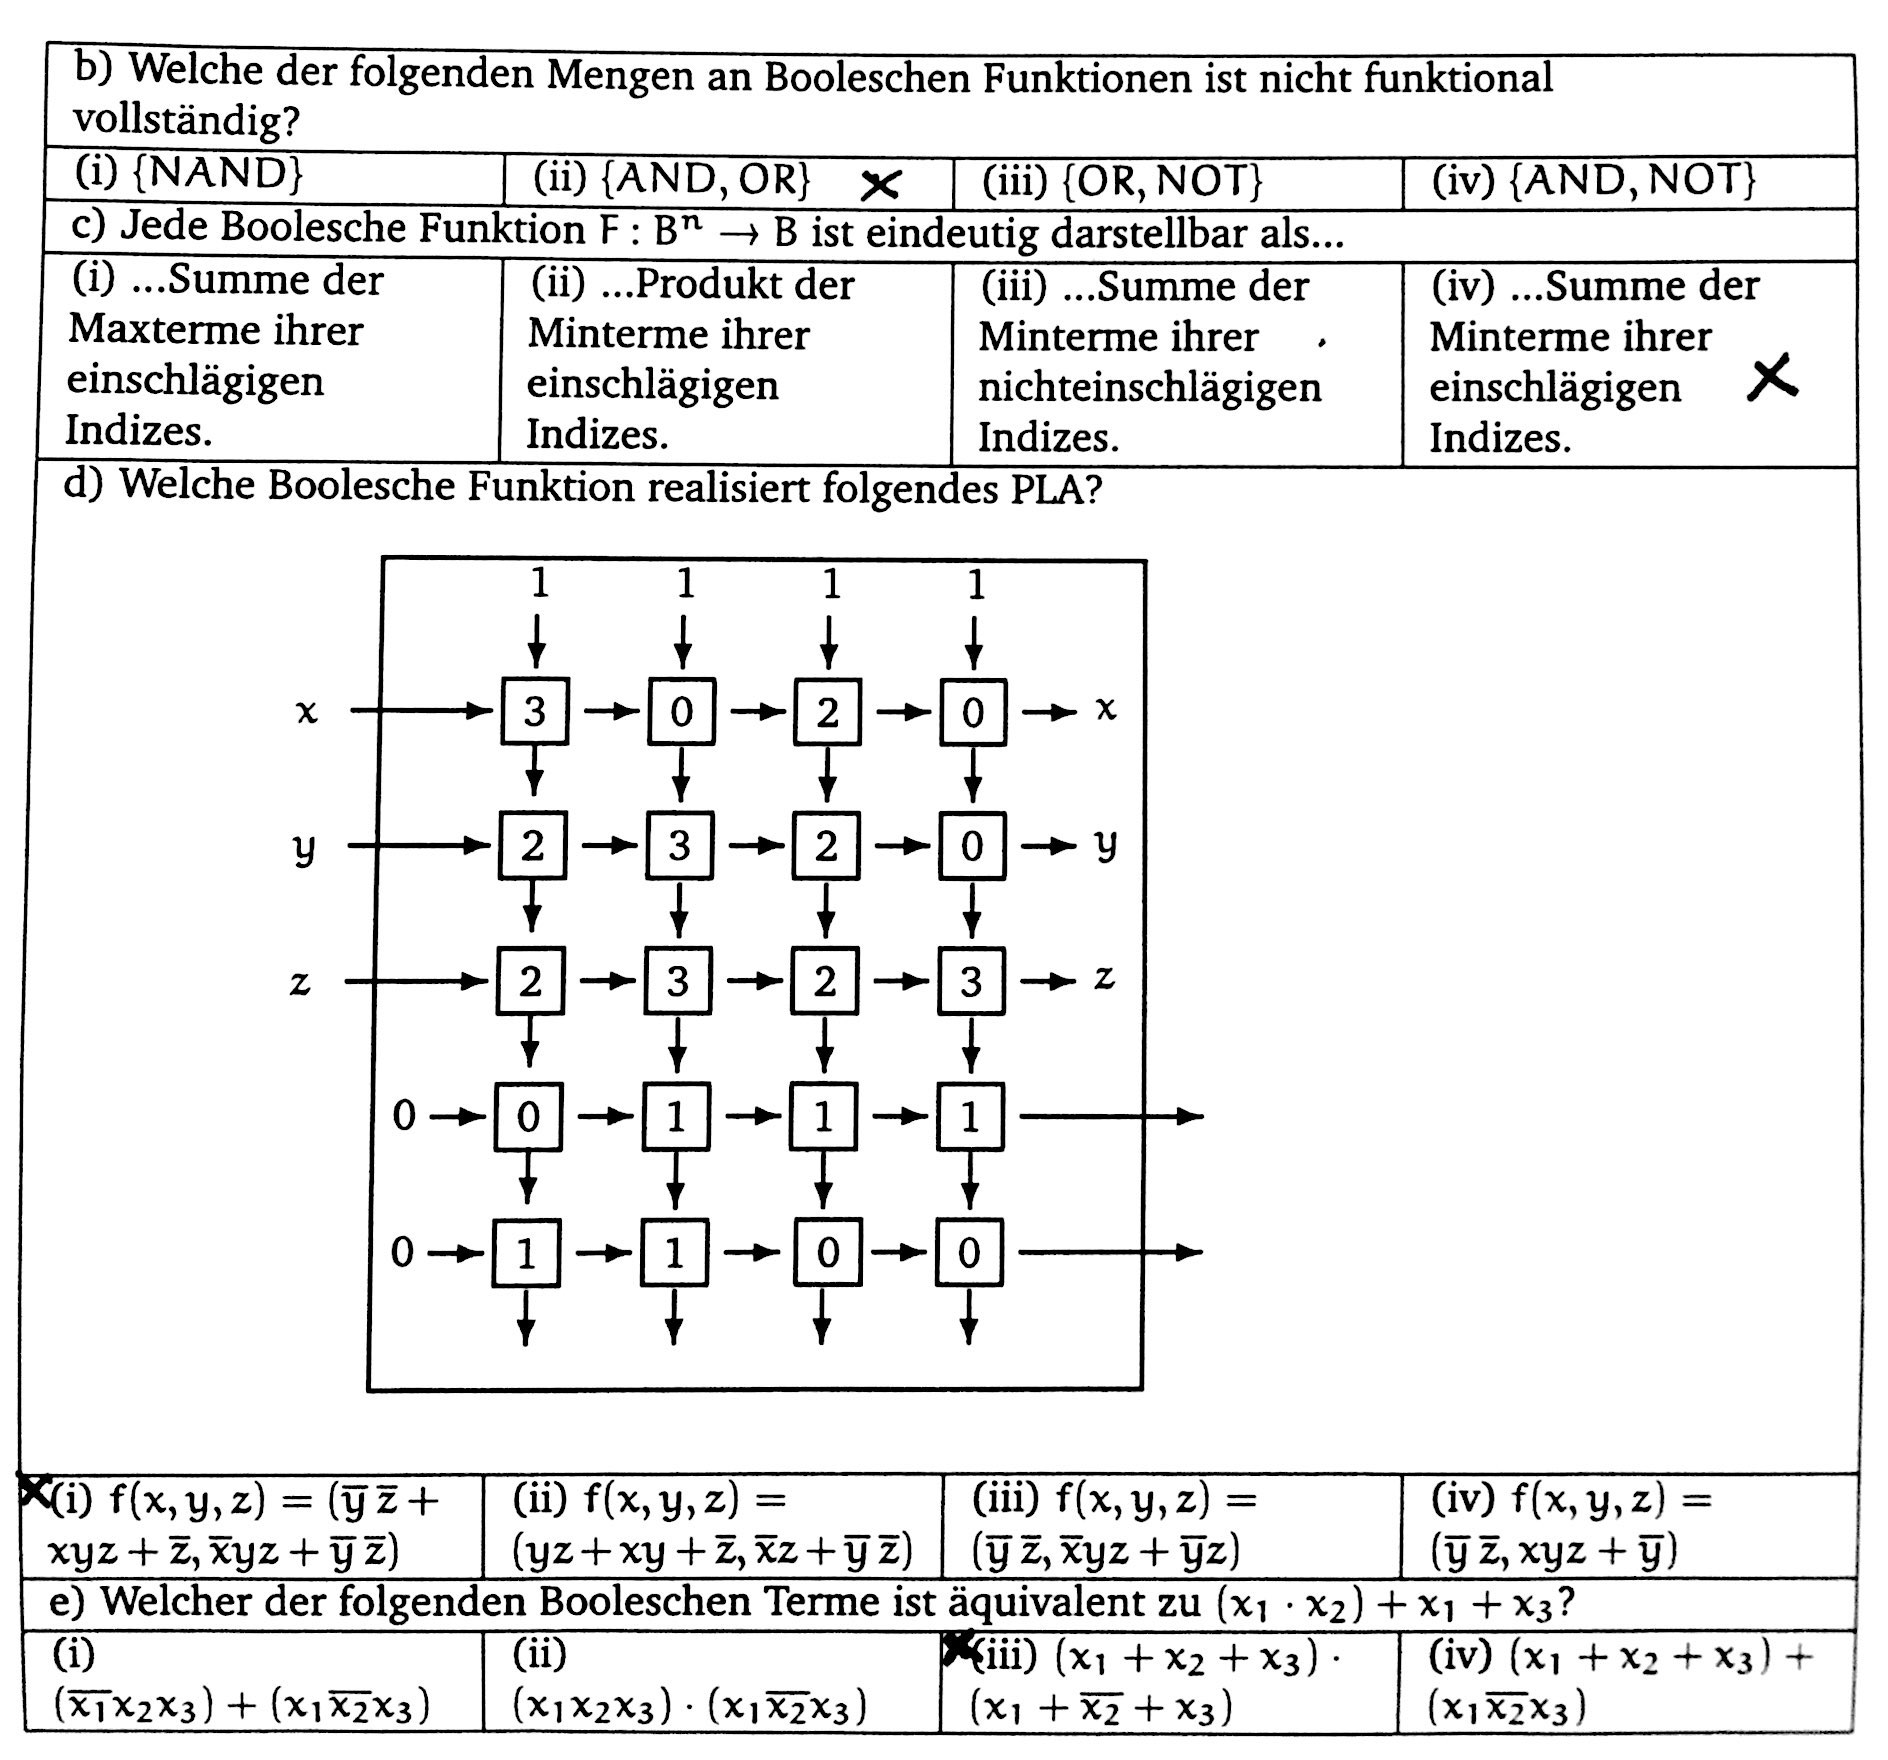
\includegraphics[scale=0.21]{d.jpg} 

\end{document}